\documentclass[tikz,border=3pt]{standalone}
\usetikzlibrary{positioning,arrows.meta,shapes.geometric,backgrounds}

\begin{document}

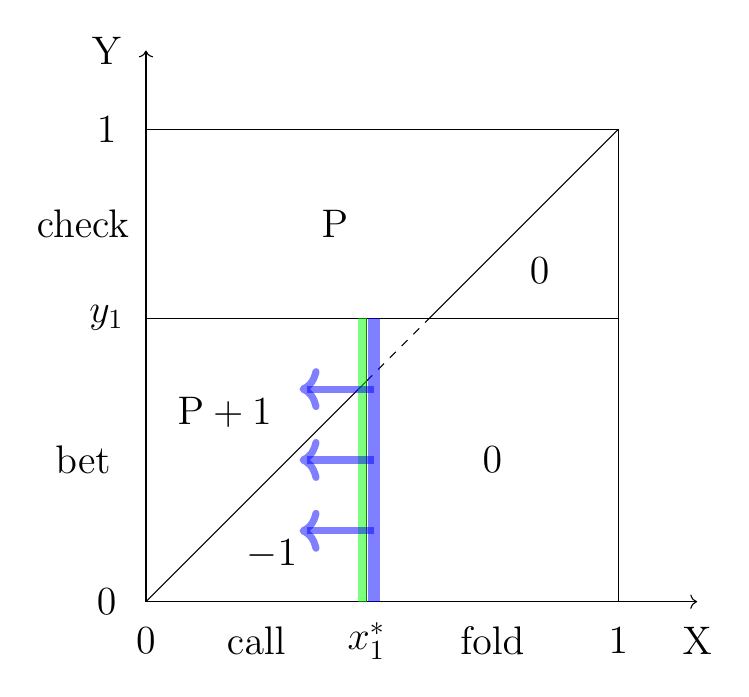
\begin{tikzpicture}

%%% 定型
\draw[->] (0,0) --(0,7);
\draw[->] (0,0) --(7,0);
\draw (0,6) --(6,6) --(6,0);

\node[font=\Large] at (7,-0.5) {X};
\node[font=\Large] at (-0.5,7) {Y};

\node[font=\Large] at (0,-0.5) {$0$};
\node[font=\Large] at (6,-0.5) {$1$};
\node[font=\Large] at (-0.5,0) {$0$};
\node[font=\Large] at (-0.5,6) {$1$};
%%%

%% 線
\draw (0,3.6) --(6,3.6);
\draw (2.8,0) --(2.8,3.6);

\draw (0,0) --(2.8,2.8);
\draw[dashed] (2.8,2.8) --(3.6,3.6);
\draw (3.6,3.6) --(6,6);

\draw[color=green, opacity=0.5, line width=1.2mm] (2.75,0) --(2.75,3.6);
\draw[color=blue, opacity=0.5, line width=1.5mm] (2.9,0) --(2.9,3.6);
\draw[->, color=blue, opacity=0.5, line width=0.9mm] (2.9,1.8) --(1.95,1.8);
\draw[->, color=blue, opacity=0.5, line width=0.9mm] (2.9,2.7) --(1.95,2.7);
\draw[->, color=blue, opacity=0.5, line width=0.9mm] (2.9,0.9) --(1.95,0.9);

%% 目盛り
\node[font=\Large] at (2.8,-0.5) {$x_1^*$};
\node[font=\Large] at (-0.5,3.6) {$y_1$};

%% 数字
\node[font=\Large] at (2.4,4.8) {$\mathrm{P}$};
\node[font=\Large] at (5.0,4.2) {$0$};
\node[font=\Large] at (4.4,1.8) {$0$};
\node[font=\Large] at (1,2.4) {$\mathrm{P}+1$};
\node[font=\Large] at (1.6,0.6) {$-1$};

%% 範囲説明
% X axis
\node[font=\Large] at (1.4,-0.5) {call};
\node[font=\Large] at (4.4,-0.5) {fold};
% Y axis
\node[font=\Large] at (-0.8,4.8) {check};
\node[font=\Large] at (-0.8,1.8) {bet};

\end{tikzpicture}
\end{document}
